\documentclass{article}
\usepackage{graphicx} % Required for inserting images
\usepackage{amsmath}
\usepackage{amssymb}
\usepackage[a4paper, total={7.5in, 10.85in}]{geometry}

\title{The Power of the Complex Plane}
\author{By Lily Sun}
\date{December 2023}

\begin{document}

\maketitle
One day, you find yourself in a dungeon. Looking around, you see the lock to get out. Underneath the lock, there is a puzzle: \\

\textit{\textbf{"There are two pegs placed at coordinates $A = (3, 1)$ and $B = (8, 13)$. Point $C$ is placed on the coordinate grid such that $\triangle ABC$ is a 5-12-13 triangle, where $AB = 13, BC = 5, AC = 12$. Give the coordinates of $C$." (Note that there are four ways to place $C$. Please give the coordinates of $C$ roughly as shown in the diagram).}} \\

\begin{center}
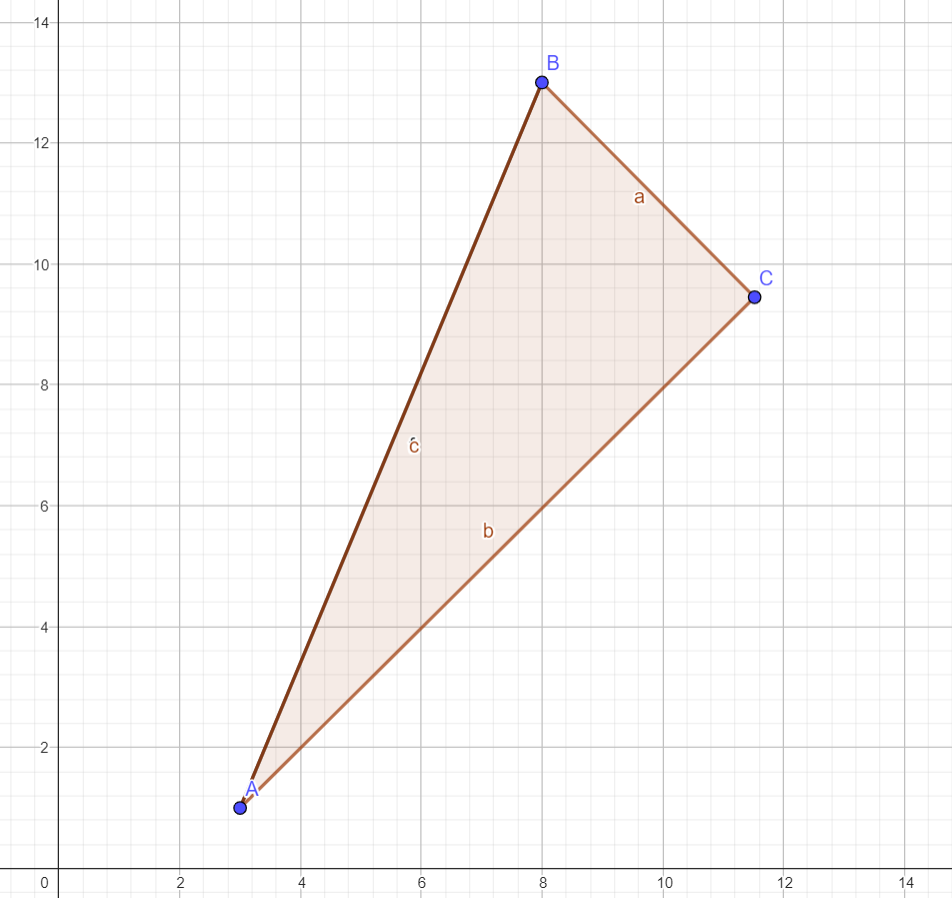
\includegraphics[scale = 0.5]{images/A3_1.png} \\
\end{center}

Intrigued by the puzzle, you wonder if there was a way to perform a rotation and dilation on $\overline{AB}$ such that you create $\overline{AC}$, one of the legs of the triangle. Then, it hits you: use the complex plane! The coordinates $(x, y)$ on the coordinate plane correspond to the point $x + yi$ on the complex plane. Namely, the x-value corresponds to the real component and the y-value corresponds to the imaginary component. The point $x+yi$ is written in rectangular form, and has nice properties when dealing with rotations and dilations. For examples, rotations can be dealt with using Euler's Formula.

\section{Rotations on the Complex Plane}

Euler's Formula states that 

$$e^{\theta i} = \cos{\theta} + i\sin{\theta}.$$

Unfortunately, a proof of this formula will be beyond the scope of this article.\\

Let's say that you have the point $e^{\alpha i}$. In rectangular form, the point is expressed as $\cos{\alpha} + i\sin{\alpha}$. On the complex plane, this is the same point as the angle $\angle{\alpha}$ on the unit circle in the complex plane. To get from angle $\alpha$ to angle $\alpha + \beta$, we need perform a transformation on $e^{\alpha i}$ such that the argument (the angle) becomes $\alpha + \beta$. By complex number multiplication, we multiply $e^{\beta i}$ to $e^{\alpha i}$ to get $e^{(\alpha + \beta) i}$. Thus, to rotate point $e^{\alpha i}$ counterclockwise about the origin by $\angle{\beta}$, we multiply it by $e^{\beta i}$, or $\cos{\beta} + i\sin{\beta}$. \\

\section{Dilations on the Complex Plane}

Now, let's explore dilations. Let's start again with a point on the complex plane, namely, $me^{\alpha i} = m(cos{\alpha} + i\sin{\alpha})$. Since the magnitude of $\cos\alpha + i\sin{\alpha}$ is $1$, the magnitude of $m(cos{\alpha} + i\sin{\alpha})$ is $m$. We want to dilate the point such that the magnitude is now $n$. Thus, we multiply by $\dfrac{n}{m}$ to get

\begin{align*}
\dfrac{n}{m} |m\cos\alpha + \sin{\alpha}i| &= \dfrac{n}{m} \cdot m,\\
\dfrac{n}{m} \cdot me^{\alpha i} &= n.\\
\end{align*}

Thus, to dilate a point $me^{\alpha i}$ such that the magnitude becomes $n$, we multiply it by $\dfrac{n}{m}$.

\section{Solving the Puzzle}

With the power of the complex plane, we are able to rotate and then dilate $\overline{AB}$ to create $\overline{AC}$. To rotate $\overline{AB}$, we first transform $\overline{AB}$ such that $A$ lies on the origin. Otherwise, we are rotating $B$ around the origin, instead of $B$ with respect to $A$. Thus, we subtract $(3, 1)$ from all points to get that $A' = (0, 0)$ and $B' = (5, 12)$. Then, we translate this onto the complex plane to get that $A' = 0$ and $B' = 5+12i$. \\ 

\begin{center}
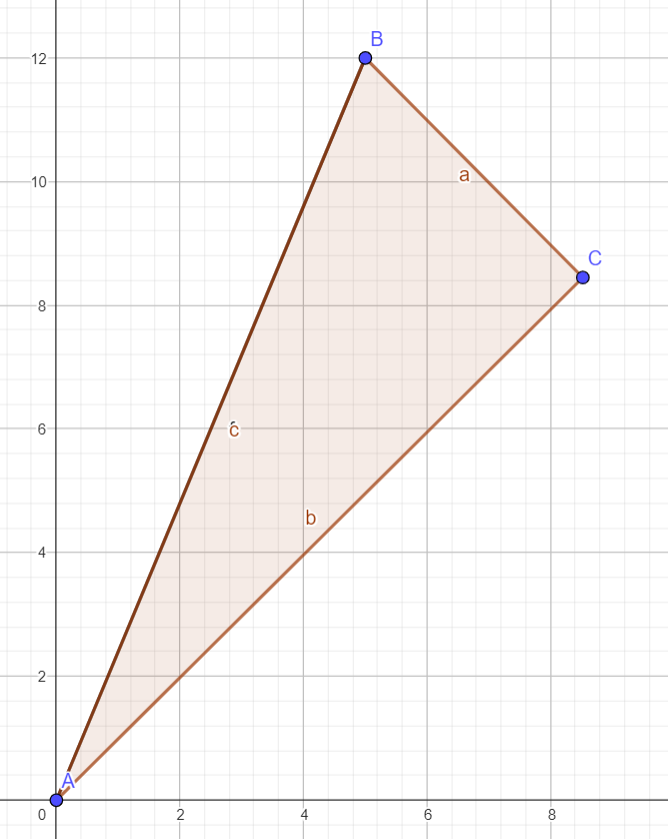
\includegraphics[scale = 0.5]{images/A3_2.png} \\
\end{center}

To rotate $\overline{AB}$ to $\overline{AC}$, we need to rotate by angle $\angle{BAC}$ clockwise around the origin. Let $\angle{BAC}$ be $\theta$. Since $\angle{ACB} = 90^{\circ}$, $\cos{\theta} = \dfrac{12}{13}$ and $\sin{\theta} = \dfrac{5}{13}$. However, since we are rotating by an angle clockwise, we are multiplying by $e^{\theta i}$. On the unit circle, a negated angle has the same cosine but opposite sine. Thus, $e^{-\theta i} = \cos{\theta} - \sin{\theta} = \dfrac{12}{13} - \dfrac{5}{13}i$ . Then, we are multiplying $5 + 12i$ by $e^{-\theta i} = \dfrac{12}{13} - \dfrac{5}{13}i$. Simplifying, we get

$$(5+12i)\left(\dfrac{12}{13} - \dfrac{5}{13}i\right) = \dfrac{120}{13} + \dfrac{119}{13}i.$$

Next, we dilate $B'$ such that magnitude matches that of what $C'$ should be. Since $|B'| = 13$ and $|C'| = 12$, we multiply $\dfrac{120}{13} + \dfrac{119}{13}i$ by $\dfrac{12}{13}$ to get that the coordinates of $C'$ are 

$$\dfrac{1440}{169} + \dfrac{1428}{169}i.$$

Lastly, we translate $C'$ back to the original spot by adding $A$, or $3+i$ to every coordinate to get that the coordinates of $C$ in rectangular form are

$$\dfrac{1947}{169} + \dfrac{1597}{169}i.$$

Thus, the coordinates of $C$ on the coordinate plane is $\left(\dfrac{1947}{169}, \dfrac{1597}{169}\right)$. Suddenly, a floating iPad comes into existence in front of you, just in time for you to type in the coordinates and open the door. We have conquered a puzzle using the power of the complex plane!

\end{document}
